
\section{序論}
小傾角粒界エネルギーにおいて,原子間ポテンシャルを用いたシミュレーションの結果と大槻による実験結果に矛盾が存在する.両者の具体的な相違点は,図に示したAlの(001)方位の粒界エネルギーの角度依存性から読み取ることができる.TschoppとMcdowellによるシミュレーション結果では,0度及び90度付近における対称傾角粒界エネルギーの立ち上がりがそれぞれ異なる傾きになっている["Asymmetric tilt grain boundary structure and energy in copper and aluminium", M. A. Tschopp and D. L. Mcdowell, Phil. Mag., Vol. 87 (2007), 3871–3892.].
その一方,大槻の実験結果では,0度及び90度付近の対称傾角粒界エネルギーの傾きが左右対称になった[A. Otuki, J. Material Science, 40(2005), 3219.].

\begin{figure}[htbp]\begin{center}
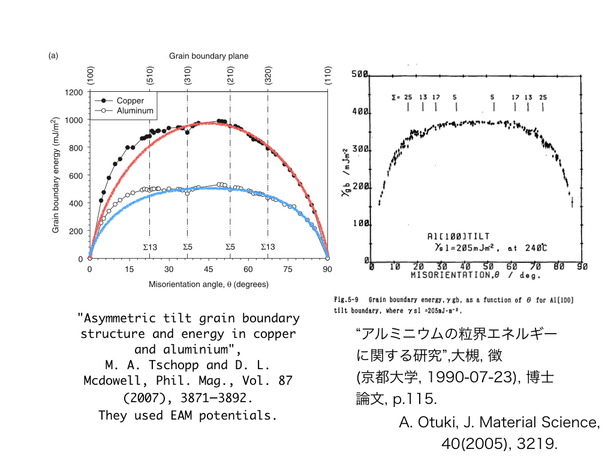
\includegraphics[width=10cm,bb= 0 0 737 553]{../figs/./boundary_narita.002.jpeg}
\caption{Al(001)対称傾角粒界エネルギーのシミュレーションと実験結果の比較.}
\label{default}\end{center}\end{figure}
Hassonらによるシミュレーションは,Read-Shockleyの理論予測をもとにおこなった.Read-Shockleyの式は以下のようになる[3].

\begin{figure}[htbp]\begin{center}
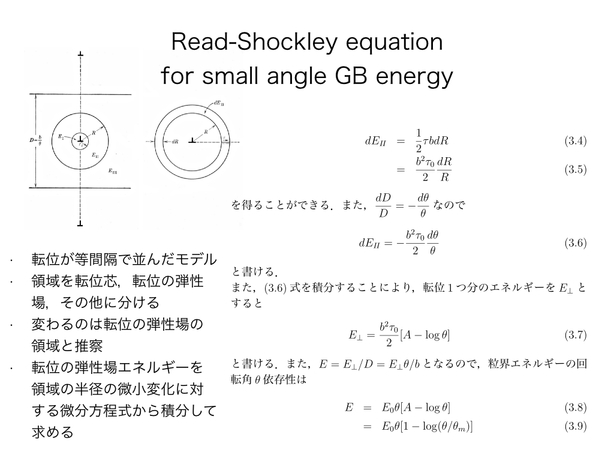
\includegraphics[width=10cm,bb= 0 0 737 553]{../figs/./boundary_narita.003.jpeg}
\caption{Read-Shockleyの理論予測.}
\label{default}\end{center}\end{figure}
小傾角粒界エネルギーによる2つの結果の矛盾を明白にするために,西谷研究室において様々な検証が今までおこなわれてきた.はじめに,第一原理計算ソフトVASPによる計算をおこない,その後,原子間ポテンシャルを使ったシミュレーションやSutton Vitekによる粒子モデルの研究を取り組んできた[1].また,八幡の研究では,経験的原子間ポテンシャルによるシミュレーションをおこない,Read-Shockleyの理論予測と同様の結果となった[2].さらに,岩佐の研究では,最安定な原子配置を探索するために原子の削除操作を取り入れ,第一原理計算ソフトVASPを用いて構造緩和し,系全体のエネルギー計算をおこなった[Iwasa].その結果,小傾角粒界エネルギーが予測通りに大槻の結果よりも低いエネルギーの値となり,粒界エネルギーの立ち上がり0度付近が最安定の構造になった.しかしながら,図{図:004}のように原子が全体的に傾いた構造になり,粒界がより低い角度になった状態を計算していた.

\begin{figure}[htbp]\begin{center}
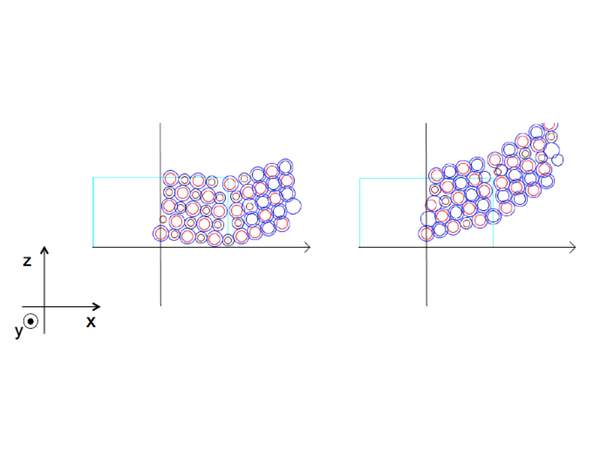
\includegraphics[width=10cm,bb= 0 0 737 553]{../figs/./boundary_narita.004.jpeg}
\caption{岩佐による誤った構造緩和の結果}
\label{default}\end{center}\end{figure}
エネルギー計算による誤った構造緩和は,安定構造の原子配置を視覚的に確認しなかったことが原因である[3].原子配置の確認はMedeaやVESTAなどの汎用モデル構築ソフトで行われていた.しかし,結果の視覚的な確認には手間がかかるため,日頃のルーチンとしては組み込まれていなかった.この失敗の原因を踏まえて,粒界原子配列を容易に視覚化できるソフトを開発することが本研究の目標である.特に,本研究では小傾角粒界の原子配置の視覚化に特化したソフトを開発する.

